\begin{animateinline}[final,autoplay,loop,controls,poster=last]{1}
    \multiframe{5}{iCOUNT=1+1}{
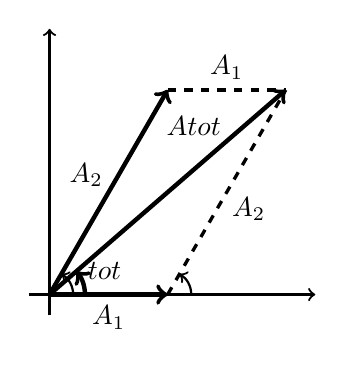
\begin{tikzpicture}[scale=0.75]
\pgfmathsetmacro{\AUN}{2.0}
\pgfmathsetmacro{\ADEUX}{4}
\pgfmathsetmacro{\PHI}{60}
\pgfmathsetmacro{\ATOT}{sqrt(\AUN^2+\ADEUX^2+2*\AUN*\ADEUX*cos(\PHI))}
\pgfmathsetmacro{\PHITOT}{acos(-(\ADEUX^2 - \AUN^2 - \ATOT^2)/(2*\AUN*\ATOT) ) }
\pgfmathsetmacro{\HMAX}{4.5}
\draw [->,thick] (0,-10pt) -- (0,\HMAX) ;
\draw [->,thick] (-10pt,0) -- (\HMAX,0) ;
\draw [->,ultra thick] (0,0) -- (\AUN,0) node [pos=0.5,below] {$A_1$};
\ifthenelse{\iCOUNT > 1}{
  \draw [->,ultra thick] (0,0) -- ({\ADEUX*cos(\PHI)},{\ADEUX*sin(\PHI)}) node [pos=0.5,above left=-2pt] {$A_2$};
  \ifthenelse{\iCOUNT < 4}{
    \draw [->,thick] (0.4,0) arc (0:\PHI:0.4) node [right] {$\ph$} ;
  }{}
  \ifthenelse{\iCOUNT > 2}{
    \draw [very thick,dashed] ({\ADEUX*cos(\PHI)},{\ADEUX*sin(\PHI)}) --++ (\AUN,0) node [pos=0.5,above] {$A_1$};
    \draw [very thick,dashed] (\AUN,0) --++ ({\ADEUX*cos(\PHI)},{\ADEUX*sin(\PHI)}) node [pos=0.5,below right=-2pt] {$A_2$};
    \draw [->,thick] ({\AUN+0.4},0) arc (0:\PHI:0.4) node [right] {$\ph$} ;
  }{}
  \ifthenelse{\iCOUNT > 3}{
    \draw [->,ultra thick] (0,0) -- ({\ADEUX*cos(\PHI)+\AUN},{\ADEUX*sin(\PHI)}) node [pos=0.75,above left=-2pt] {$A\e{tot}$};
    \draw [->,ultra thick] (0.6,0) arc (0:\PHITOT:0.6) node [right] {$\ph\e{tot}$} ;
  }{}
}{}
\end{tikzpicture}
}
\end{animateinline}

